%!TEX root=../ctl-phd-thesis.tex

\section{Supplementary Information}
    \subsection{Langevin Dynamics Engine}
        \par We have developed a software package which performs Langevin dynamics calculations on a user specified PMF and diffusivity profile. The engine is implemented using the Python and C programming languages. To run a simulation the user specifies a PMF and viscosity profile as well as the hydrodynamic radius and mass.

        \par The PMF profile is generated using a piecewise cubic Hermite polynomial (PCHIP) from the following user-specified values: \texttt{dz}, the distance from the center to the edge of the membrane; \texttt{W1}, \texttt{W2}, and \texttt{W3}, the PMF at the interface, between the interface/core, and at the core of the membrane respectively; as well as \texttt{a} and \texttt{b} which correspond to the location of the water bilayer interface and interface/core.  We interpolate the points using \texttt{scipy.interpolate}. Conveniently the PCHIP algorithm allows for both fast computation of the value at any point. Furthermore we can precalculate the first derivative, the negative value of which is the force, as another spline for fast evaluation. The viscosity profile is computed in a similar fashion though requiring additional inputs: \texttt{dz}, the distance from the center to edge of the membrane; \texttt{d1}, \texttt{d2}, \texttt{d3}, and \texttt{d4}, the viscocities in bulk, the interface, interface/core, and core respectively; and \texttt{a}, \texttt{b}, \texttt{c} which specify the location of the interface, interface/core, and core respectively.

        \par The Gr\o nbach-Jensen--Farago integrator is implemented in both Python and C. To generate Gaussian random number in C, we employ the use of the PCG random number generator (RNG)~\cite{ONeill} to sample random integers. These random integers are converted to random uniform floating point numbers by using a bit stream algorithm by Taylor R. Campbell. Uniform floats are then transformed using the Box-Muller algorithm to yield a gaussian random number. The qualities of our C random number generator are compared to that of python library \texttt{numpy} in fig.~\ref{fig:testRNG}. The numpy and C RNGs are seeded off entropy from \texttt{/dev/urandom}. The C integrator is wrapped using the Python/C API allowing it to be called from Python which handles the system setup, configuration, and analysis.

        \begin{figure}[!htbp]
        \begin{center}
            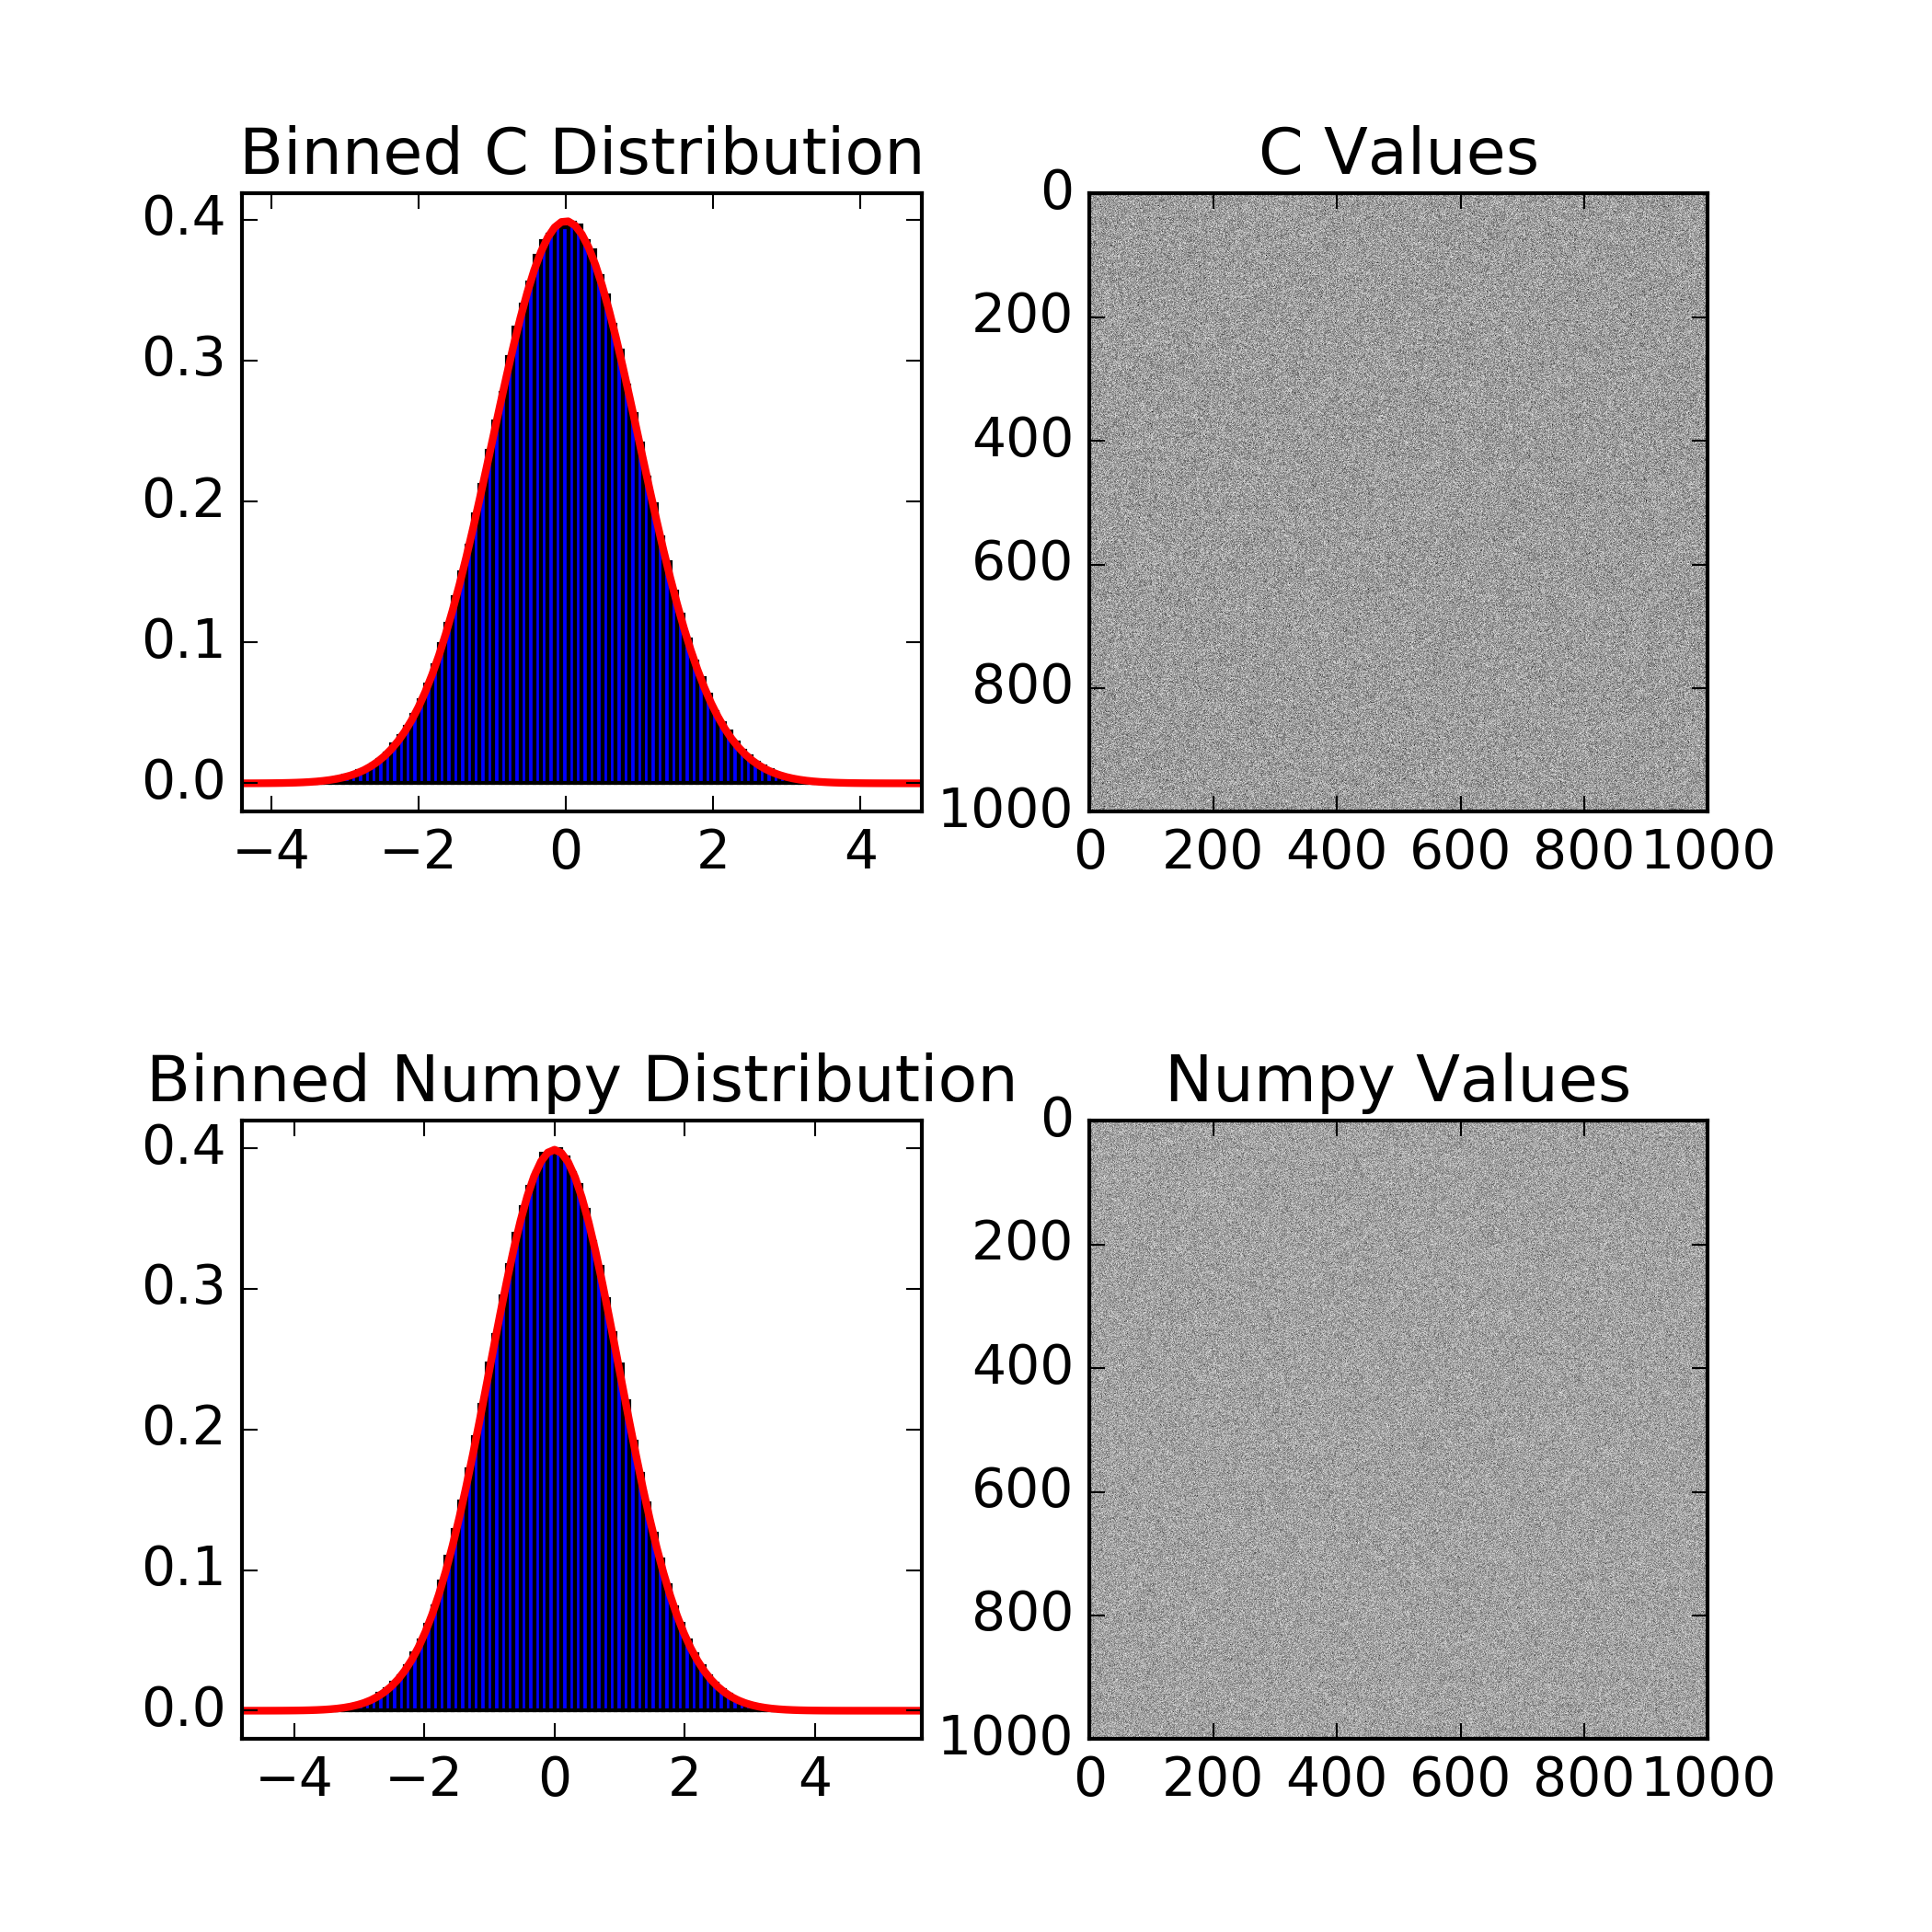
\includegraphics[width=0.8\textwidth]{Figures/testRNG}
            \caption[Randomness of gaussian random numbers]{The binned probability distribution of both C and \texttt{numpy} generated gaussian random numbers are shown in comparison with an ideal Gaussian with zero mean and unit variance. On the right, a greyscale plot of the sequence of random numbers indicates, by visual inspection, that they are not correlated and there are no repeat sequences.}
            \label{fig:testRNG}
        \end{center}
        \end{figure}

    \subsection{Milestoning Sampling and Efficiency}
        \par The total number of statistics aggregated during milestoning for each system is shown in fig.~\ref{fig:transitions}. Notably, the statistics consist of only the trajectories which were members of the first hitting point distribution (FHPD). To quantify the efficiency of identifying FHPD members we ran a quick test of the accept rate of the milestone at $z=0$ with adjacent milestones at $z=-1,1$ for 10000 random members with a timestep of $1\times 10^{-15}$~s. We find that the typical rejection rate is upwards of $\approx$90\% (9000) during the reverse phase. While most rejections come about from self-crossing events occurring in the first several timesteps, and thus contribute little to the total computer time, the number of trajectories required to generate a well-explored FHPD is very large, making the compute time of rejections non-trivial. None of the reported statistics account for the number of rejected trajectories.

        \begin{figure}[!htbp]
        \begin{center}
            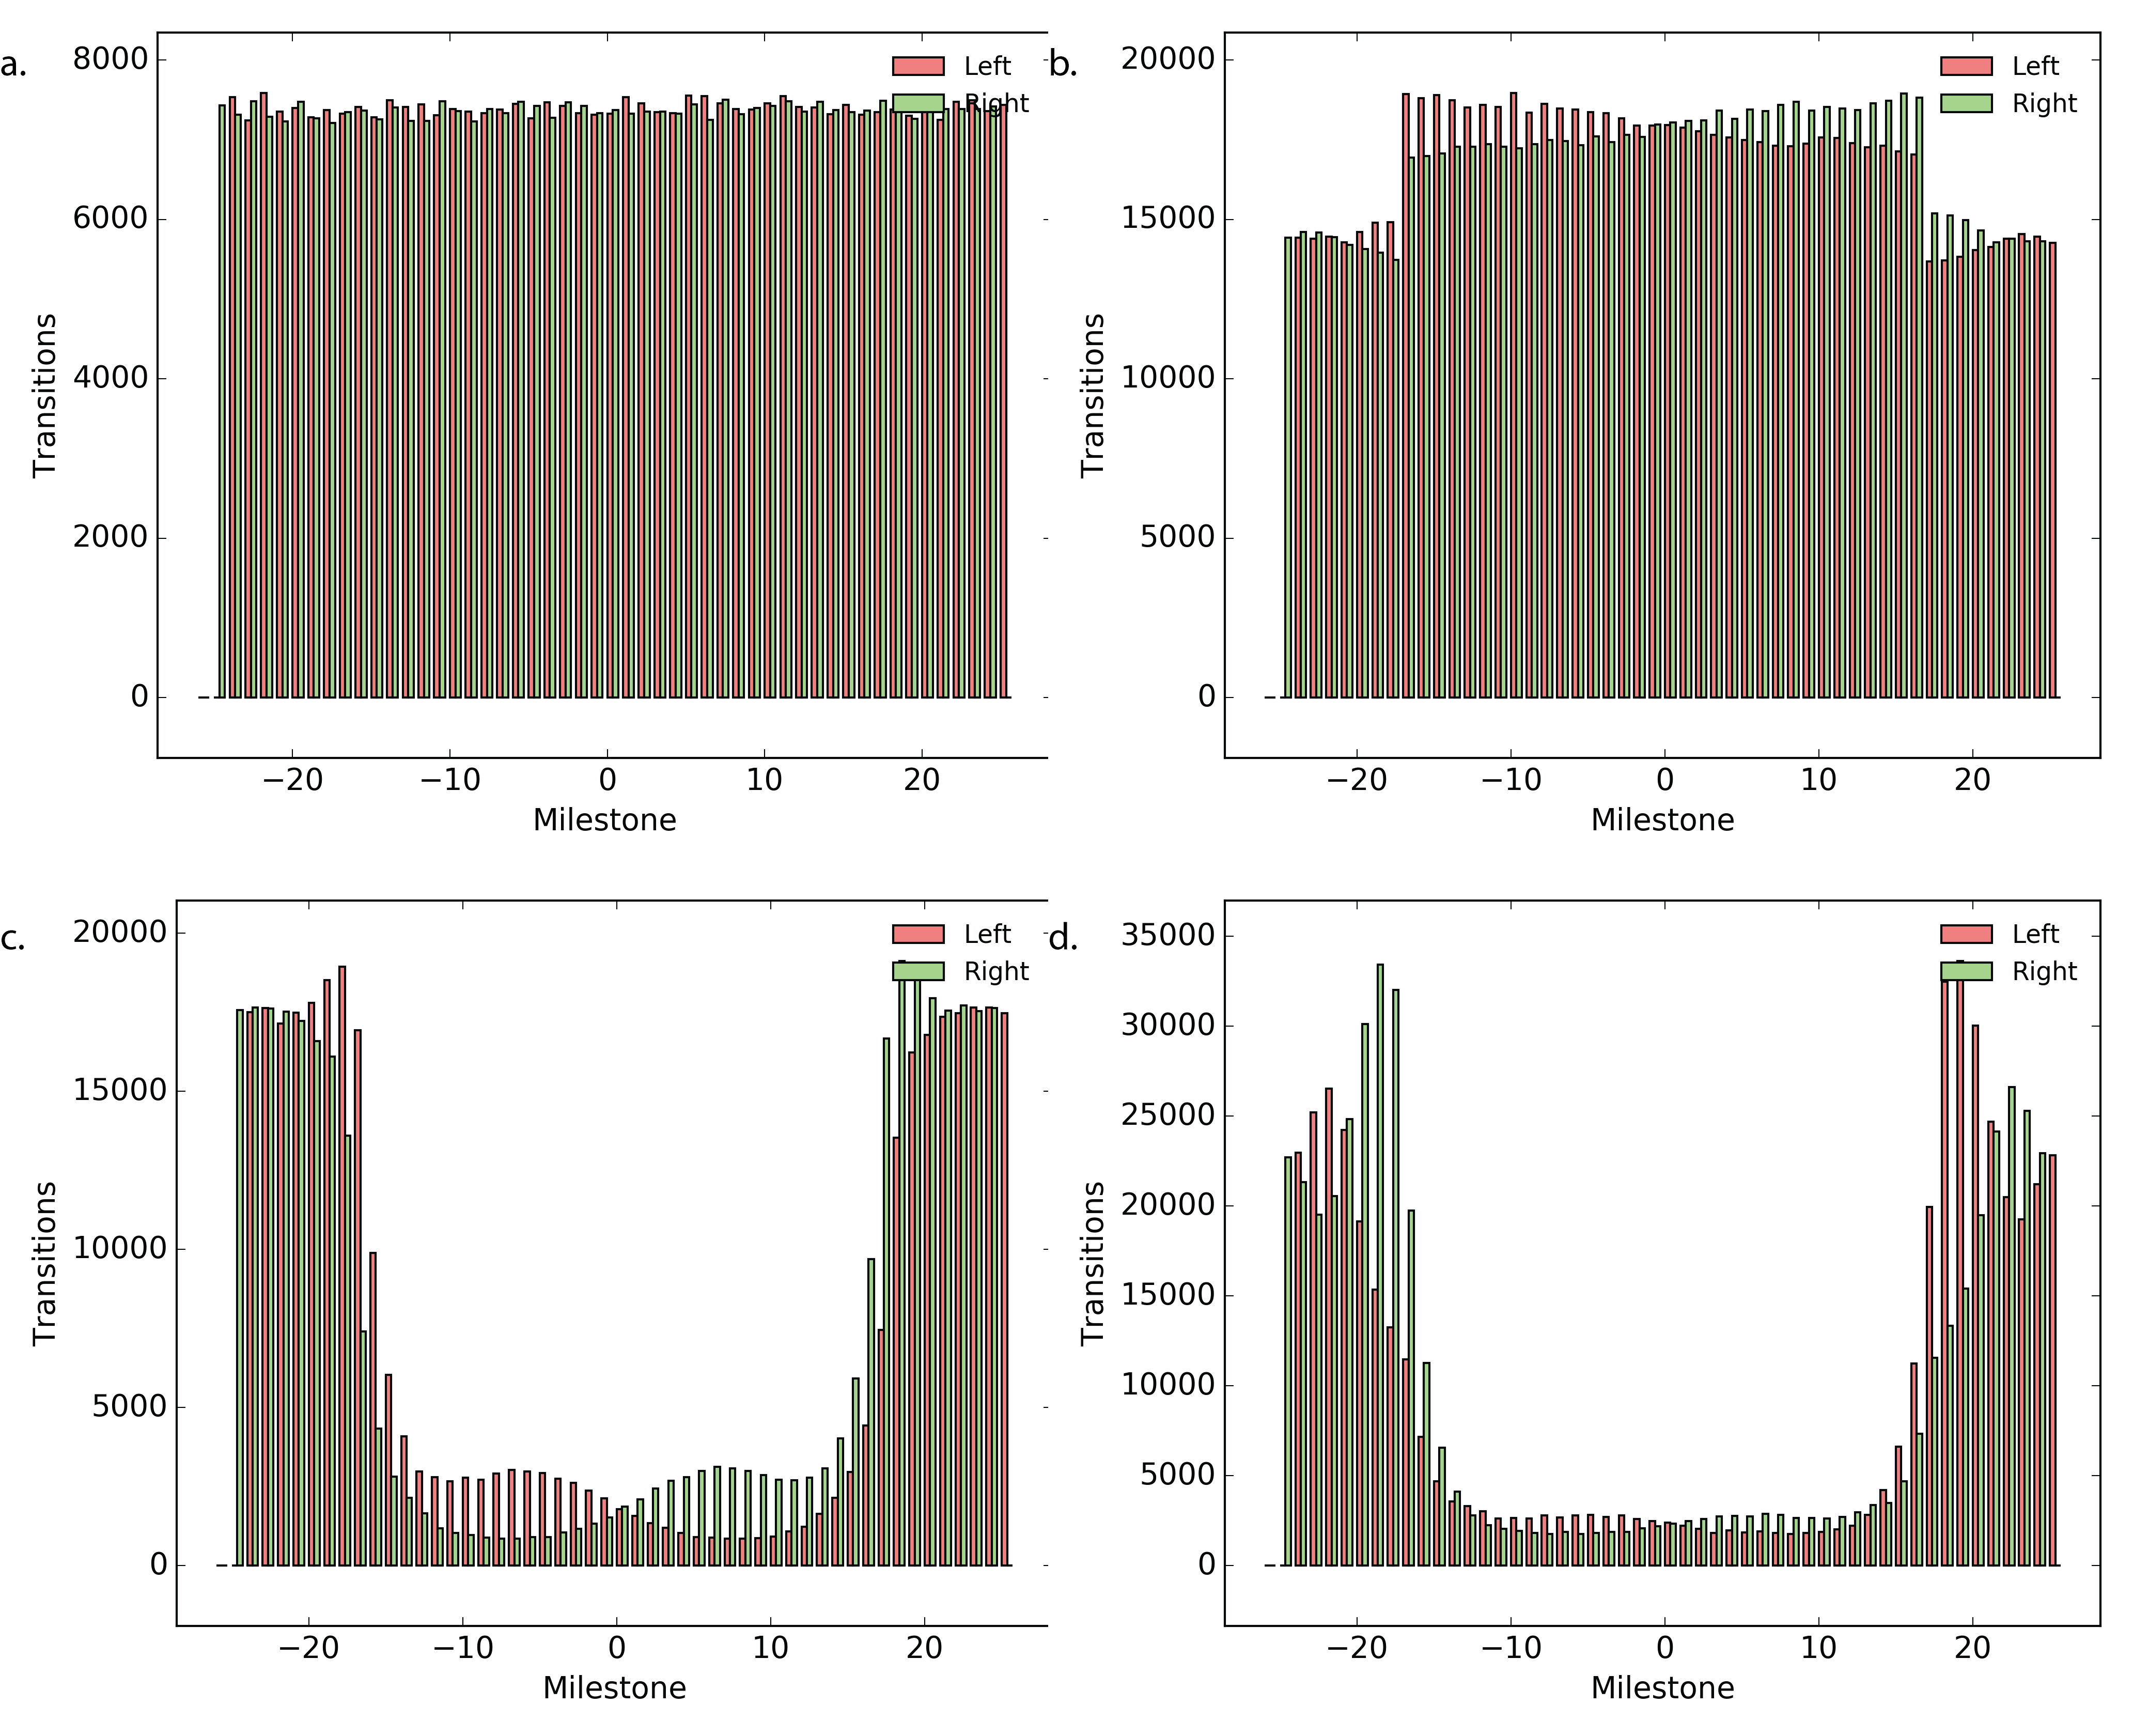
\includegraphics[width=0.8\textwidth]{Figures/transitions}
            \caption[Number of forward and reverse trajectories collected for each toy system]{Shown here are the total number of forward and reverse trajectories collected for systems (a) flat, (b) small-barrier, (c) urea, and (d) codeine.}
            \label{fig:transitions}
        \end{center}
        \end{figure}

    \subsection{Sampling Convergence of Crossing Probabilities}
        \par To quantify the impact of sampling on our confidence in crossing probability, we compute the 95\% confidence of $\rho=0.5$ with respect to a total number of observations. Confidence intervals are estimated using the percentile boostrap over 10,000 resamples. The results are shown in fig.~\ref{fig:bootRho}. Even at $N=200$ the confidence interval is still quite large at $0.07$. The calculation of $\rho$ is a binomial sampling problem, thus the 95\% confidence interval should follow the following solution,
        \begin{equation}
            CI(95) = 2\rho/\sqrt{N-1}.
        \end{equation}

        \begin{figure}[!htbp]
        \begin{center}
            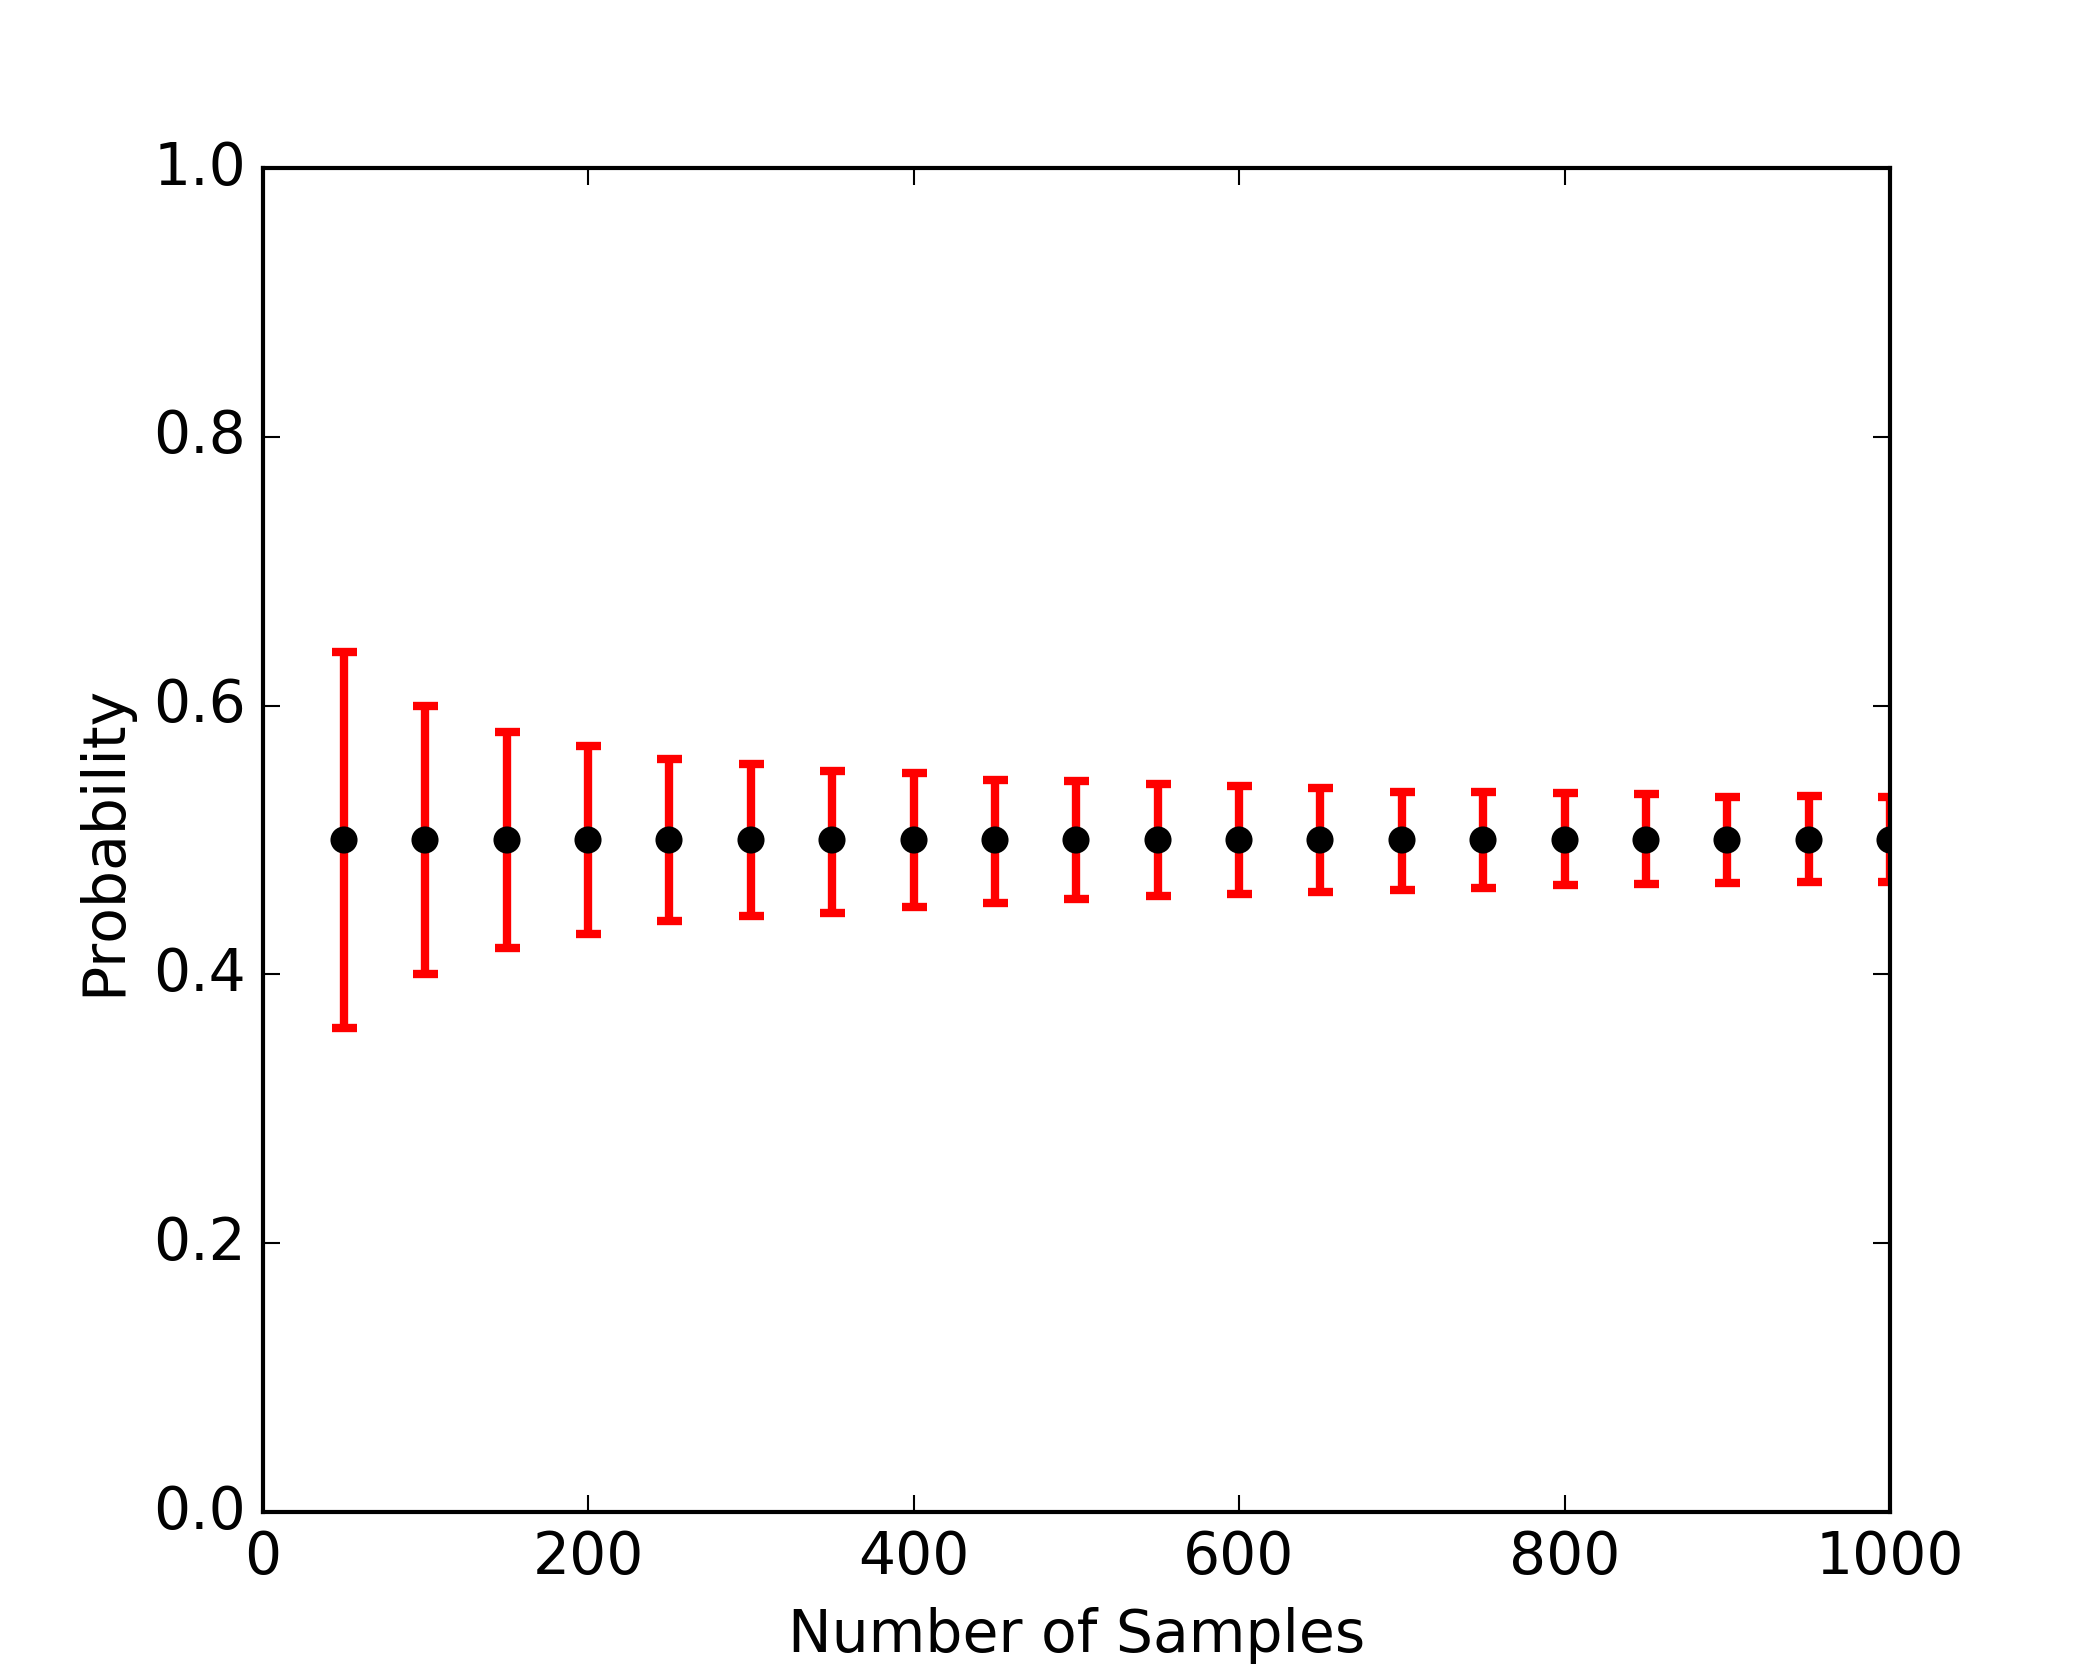
\includegraphics[width=0.8\textwidth]{Figures/bootRho}
            \caption{The 95\% confidence intervals of a 50-50 crossing probability with respect to the total number of observations.}
            \label{fig:bootRho}
        \end{center}
        \end{figure}
